\section{Einleitung}

Ziel dieses Versuchs ist die experimentelle Bestätigung der Geschwindigkeitsgleichung für die säurekatalysierte Iodierung von Aceton.
Dies erfolgt durch die Bestimmung der Teilordnungen $a$, $b$, und $c$ bezüglich Aceton [A], Oxonium-Ionen \ch{H3O+}, und Iod \ch{I2} mittels der Methode der variierten Anfangsgeschwindigkeiten.
Des Weiteren soll die Geschwindigkeitskonstante $k_{exp}$ für unterschiedliche Temperaturen ermittelt und daraus die Aktivierungsenergie $E_A$ bestimmt werden.

\section{Theoretische Grundlagen}

\subsection{Reaktionsmechanismus}

Die Iodierung von Aceton ist eine säurekatalysierte Reaktion, die in drei Teilschritten abläuft.
\begin{enumerate}
    \item Protonierung des Acetons [A] (schnelles Gleichgewicht).
    \item Enolisierung des protonierten Acetons zum Enol [E] (geschwindigkeitsbestimmender Schritt).
    \item Reaktion des Enols mit Iod zum Produkt (schnelle Reaktion).
\end{enumerate}

\begin{scheme}
    \centering
    \schemestart
    \setchemfig{atom sep=2em}
    \chemfig{H_{3}C-C(=[6]O)-CH_{3}} + \ch{I2} \ch{ ->[ H+ ]} \chemfig{H_{3}C-C(=[6]O)-CH{2}I} + \ch{HI}
    \schemestop
    \caption{Säurekatalysierte Iodierung von Aceton.}
\end{scheme}

Unter der Annahme, dass die Weiterreaktion des Enols mit Iod sehr viel schneller als die Rückreaktion stattfindet
\begin{equation*}
   \left(k_2 \cdot [I_2] \gg k_{-1} \cdot [H_3O^+]\right) 
\end{equation*}
ergibt sich die Reaktionsgeschwindigkeit $v$ als unabhängig von der Iod-Konzentration:

\begin{equation}
   v = \frac{d[P]}{dt} = k_{exp} \cdot [A] \cdot [H_3O^+]
\end{equation}

Die Gesamtordnung der Reaktion beträgt somit 2, mit einer 1. Ordnung bezüglich Aceton und Säure, und einer 0. Ordnung bezüglich Iod.

\subsection{Bestimmung der Reaktionsordnung}
Die allgemeine Geschwindigkeitsgleichung lautet:
\begin{equation}
    v = \frac{-d[I_2]}{dt} = k_{exp} \cdot [A]^{a} \cdot [H_3O^{+}]^{b} \cdot [I_2]^{c}
\end{equation}
Die Teilordnungen $a$, $b$, und $c$ werden durch die Methode der variierten Anfangsgeschwindigkeiten bestimmt. 
Hierbei wird die Anfangskonzentration eines Reaktionspartners variiert, während die Konzentrationen der anderen konstant gehalten werden.

Die Anfangsgeschwindigkeit $v_0$ wird durch den Differenzenquotienten approximiert, da über ein kleines Zeitintervall $\Delta t$ die Konzentrationsänderung $\Delta [I_2]$ ebenfalls klein ist:
\begin{equation}
    v_0 \approx \frac{[I_2]_0}{\Delta t} \label{eqn:anfangsgeschwindigkeit}
\end{equation}
Die Teilordnung $a$ (für Aceton) wird durch das Verhältnis der Anfangsgeschwindigkeiten zweier Versuche (1 und 2) mit unterschiedlichen $[A]$ berechnet:
\begin{equation}
    a = \frac{\log \left[\frac{v_0(1)}{v_0(2)}\right]}{\log \left[\frac{[A]_{(1)}}{[A]_{(2)}}\right]} \label{eqn:teilordnung}
\end{equation}
Die Teilordnungen $b$ und $c$ werden analog bestimmt.

\subsection{Bestimmung der Aktivierungsenergie $E_A$}
Die Temperaturabhängigkeit der Geschwindigkeitskonstante $k$ wird durch die Arrhenius-Gleichung beschrieben:

\begin{equation}
k = A \cdot e^{-\frac{E_A}{R T}}
\end{equation}

Durch Logarithmierung erhält man die linearisierte Form:

\begin{equation}
    \ln k = \ln A - \frac{E_A}{R} \cdot \frac{1}{T} \label{eqn:arrhenius-linear}
\end{equation}

Trägt man $\ln k$ gegen $1/T$ auf, ergibt sich eine Gerade, deren Steigung $m$ zur Bestimmung der Aktivierungsenergie $E_A$ dient:

\begin{equation}
m = -\frac{E_A}{R} \Rightarrow E_A = -m \cdot R
\end{equation}

wobei $R$ die allgemeine Gaskonstante ist.

\section{Durchführung}
\subsection{Materialien und Reagenzien}
\subsubsection{Geräte}
\begin{itemize}
    \item Messkolben (50 mL)
    \item Reagenzgläser
    \item Vollpipetten
    \item Stoppuhr
    \item Temperierbares Wasserbad
\end{itemize}
\subsubsection{Reagenzien}
\begin{itemize}
    \item Kaliumtriiodid-Lösung (\qty{0.01}{\mol\per\liter})
    \item HCl-Lösung (\qty{1}{\mol\per\liter})
    \item Aceton p.a. (\qty{6}{\mol\per\liter}) (selbst herzustellen)
    \item Stärke-Lösung (0.1\%)
\end{itemize}

\subsubsection{Sicherheitshinweise zu Reagenzien}
\adjustbox{raise=2em}{\mbox{\stackengine{\Sstackgap}{%
\textbf{\Large Aceton}}{\danger}{U}{l}{F}{T}{S}}}\hfill
\ghspic{exclam}\ghspic{flame} \\
\ghs*{h}{225}
\ghs*{h}{319}
\ghs*{h}{336}
\ghs*{p}{210}

\adjustbox{raise=2em}{\mbox{\stackengine{\Sstackgap}{%
\textbf{\Large Salzsäure}}{\danger}{U}{l}{F}{T}{S}}}\hfill
\ghspic{exclam}\ghspic{acid} \\
\ghs*{h}{319}
\ghs*{h}{335}
\ghs*{p}{305+351+338}

Aufgrund der starken Verdünnung der Kaliumtriiodid-Lösung gehen von dieser keine besonderen Gefahren aus.
Da Iod stark färbt, werden Handschuhe empfohlen, um Hautverfärbungen zu vermeiden.

%\adjustbox{raise=2em}{\mbox{\stackengine{\Sstackgap}{%
%\textbf{\Large Kaliumtriiodid (Lösung)}}{\warning}{U}{l}{F}{T}{S}}}\hfill
%\ghspic{exclam}\ghspic{acid} \\
%\ghs*{h}{302}
%\ghs*{h}{315}
%\ghs*{h}{319}
%\ghs*{h}{335}
%\ghs*{p}{280}

\subsection{Versuchsablauf}
Die in \autoref{tab:proben} gelisteten Volumina an Aceton-, Salzsäure-, Stärke-Lösung und Wasser wurden in einen 50 mL Messkolben pipettiert und gut durchmischt. 
Die Kaliumtriiodid-Lösung wurde in ein Reagenzglas pipettiert.

Beide Gefäße (Messkolben und Reagenzglas) werden für zehn Minuten in das temperierte Wasserbad gestellt.
Die Versuchsreihe wird bei Raumtemperatur, \qty{30}{\degreeCelsius} und \qty{35}{\degreeCelsius} durchgeführt.

Nach der Temperierung wurde die Kaliumtriiodid-Lösung zum Inhalt des Messkolbens gegeben.
Der Messkolben wird sofort gut geschüttelt und die Stoppuhr gleichzeitig gestartet.
Für den Messzeitraum verblieb der Messkolben außerhalb des Wasserbades.

Die anfängliche Farbe wechselte von grünbraun (Iod-Überschuss) über blau (Iod-Stärke-Komplex) zu farblos (alles Iod verbraucht).
Die Stoppuhr wurde angehalten, sobald die Lösung farblos wirde (Entfärbung), und der Wert ($\Delta t$) notiert.

Die Proben 1 bis 4 wurden jeweils bei den drei verschiedenen Temperaturen gemessen.
\begin{table}[H]
    \centering
    \caption{Ansatzvolumina (Proben 1-4) in \unit{\milli\liter}.}
    \begin{tabular}{c c c c c c}
        \toprule
        Probe & 6M Aceton & 1M HCl & 0{,}01M KI$_3$ & 0{,}1M Stärke & H$_2$O (Dest.\ Wasser) \\ \midrule
        1 &  5 &  5 &  5 &  1 &  9 \\ \midrule
        2 & 10 &  5 &  5 &  1 &  4 \\ \midrule
        3 &  5 & 10 &  5 &  1 &  4 \\ \midrule
        4 &  5 &  5 & 10 &  1 &  4 \\
        \bottomrule
    \end{tabular}
    \label{tab:proben}
\end{table}

\section{Ergebnisse und Auswertung}
Die Raumtemperatur wurde zum Zeitpunkt des Versuches zu \qty{22 +- 1}{\degreeCelsius} bestimmt.

Die Zeitmessungen ergaben die in \autoref{tab:zeitmessungen} dargestellten Werte für die verschiedenen Proben und Temperaturen.
Der Fehler der Zeitmessung wurde auf $\pm \qty{15}{\second}$ geschätzt, da der Farbumschlag nicht schlagartig, sondern allmählich erfolgte und sich einige Lösungen auch nicht vollständig entfärbten.
\begin{table}[H]
    \centering
    \caption{Gemessene Zeiten $\Delta t$ bis zum Farbumschlag in \unit{\second}.}
    \label{tab:zeitmessungen}
    \begin{tabular}{c c c c}
        \toprule
        Probe & $\Delta t_{RT}$ [\unit{\second}] & $\Delta t_{\qty{30}{\degreeCelsius}}$ [\unit{\second}] & $\Delta t_{\qty{35}{\degreeCelsius}}$ [\unit{\second}] \\ \midrule
        1 & \num{385 +- 15} & \num{205 +- 15} & \num{115 +- 15} \\ \midrule
        2 & \num{170 +- 15} &  \num{86 +- 15} &  \num{50 +- 15} \\ \midrule
        3 & \num{210 +- 15} & \num{140 +- 15} &  \num{52 +- 15} \\ \midrule
        4 & \num{755 +- 15} & \num{460 +- 15} & \num{265 +- 15} \\
        \bottomrule
    \end{tabular}
\end{table}

\subsection{Anfangskonzentrationen}
Beispielberechnung $[\ch{I2}]_0$ (Probe 1):
\begin{align*}
   [\ch{I2}]_0 &= c({\ch{KI3}}) \cdot \frac{V_{\ch{KI3}}}{V_{ges}} \\
               &= \qty{0.01}{\mol\per\liter} \cdot \frac{\qty{5}{\milli\liter}}{\qty{25}{\milli\liter}} \\
               &= \qty{0.0020}{\mol\per\liter}
\end{align*}
\begin{table}[H]
    \centering
    \caption{Anfangskonzentrationen der Proben 1 bis 4.}
    \label{tab:anfangskonzentrationen}
    \begin{tabular}{c c c c}
        \toprule
        Probe & $[\ch{A}]_0 / \unit{\mol\per\liter}$ & $[\ch{H3O+}]_0 / \unit{\mol\per\liter}$ & $[\ch{I2}]_0 / \unit{\milli\mol\per\liter}$ \\ \midrule
        1 & 1.2 & 0.2 & 2.0 \\ \midrule
        2 & 2.4 & 0.2 & 2.0 \\ \midrule
        3 & 1.2 & 0.4 & 2.0 \\ \midrule
        4 & 1.2 & 0.2 & 4.0 \\
        \bottomrule
    \end{tabular}
\end{table}

\subsection{Anfangsgeschwindigkeiten}
Die Anfangsgeschwindigkeiten $v_0$ werden mittels des Differenzenquotienten nach \autoref{eqn:anfangsgeschwindigkeit} berechnet.
\begin{align*}
    v_0 &\approx \frac{[\ch{I2}]_0}{\Delta t} \tag{\ref{eqn:anfangsgeschwindigkeit} Wdh.} \\
\intertext{Beispielberechnung $v_0$ (Probe 1, RT):}
    v_0 &= \frac{-\qty{0.0020}{\mol\per\liter}}{\qty{385 +- 15}{\second}} \\
        &= \qty{52.0 +- 2.1e-7}{\mol\per\liter\per\second}
\end{align*}
\begin{table}[H]
    \centering
    \caption{Berechnete Anfangsgeschwindigkeiten $v_0$ der Proben 1 bis 4 bei verschiedenen Temperaturen $T$.}
    \label{tab:anfangsgeschwindigkeiten}
    \begin{tabular}{c c c c}
        \toprule
        Probe & $v_0$ (\qty{22}{\degreeCelsius}) [\unit{\milli\mol\per\liter\per\second}] & $v_0$ (\qty{30}{\degreeCelsius}) [\unit{\milli\mol\per\liter\per\second}]
        & $v_0$ (\qty{35}{\degreeCelsius}) [\unit{\milli\mol\per\liter\per\second}] \\ \midrule
        1 & \num{52.0 +- 2.1e-4} & \num{97.6 +- 7.2e-4} & \num{17.4 +-  2.3e-3} \\ \midrule
        2 & \num{11.8 +- 1.1e-3} & \num{23.3 +- 4.1e-3} & \num{4.0 +- 1.2e-2} \\ \midrule
        3 & \num{95.2 +- 6.8e-3} & \num{14.3 +- 1.6e-3} & \num{3.9 +- 1.2e-2} \\ \midrule
        4 & \num{53.0 +- 1.1e-4} & \num{87.0 +- 2.9e-4} & \num{150.9 +- 8.6e-4} \\
        \bottomrule
    \end{tabular}
\end{table}

\subsection{Bestimmung der Teilordnungen}\label{sec:teilordnung}
Die Teilordnungen $a$, $b$, und $c$ werden nach \autoref{eqn:teilordnung} durch die Methode der variierten Anfangsgeschwindigkeiten bestimmt.
Hierzu werden zunächst die Teilordnungen für die verschiedenen Temperaturen einzeln berechnet und anschließend gemittelt.
Die berechneten Teilordnungen sind in \autoref{tab:teilordnungen} gelistet.
\begin{align*}
    a &= \frac{\log \left[\frac{v_0(1)}{v_0(2)}\right]}{\log \left[\frac{[A]_{(1)}}{[A]_{(2)}}\right]} \tag{\ref{eqn:teilordnung} Wdh.} \\
    \intertext{Beispielberechnung $a$ (RT):}
    a &= \frac{\log \left[\frac{\qty{52.0 +- 2.1e-4}{\milli\mol\per\liter\per\second}}{\qty{11.8 +- 1.1e-3}{\milli\mol\per\liter\per\second}}\right]}
                {\log \left[\frac{\qty{1.2}{\mol\per\liter}}{\qty{2.4}{\mol\per\liter}}\right]} \\
    &= \num{1.18 +- 0.33}
\end{align*}
\begin{table}[H]
    \centering
    \caption{Berechnete Teilordnungen $a, b, c$ bei den verschiedenen Temperaturen $T$ (22, 30, \qty{35}{\degreeCelsius}), und deren Mittelwerte.}
    \label{tab:teilordnungen}
    \begin{tabular}{c c c c}
        \toprule
        $T$ [\unit{\degreeCelsius}] & $a$ (bzgl. Aceton) & $b$ (bzgl. \ch{H3O+}) & $c$ (bzgl. \ch{I2}) \\ \midrule
        22 & \num{1.18 +- 0.33} & \num{0.85 +- 0.28} & \num{0.028 +- 0.146} \\ \midrule
        30 & \num{1.25 +- 0.63} & \num{0.55 +- 0.42} & \num{-0.17 +- 0.27} \\ \midrule
        35 & \num{1.2 +- 1.1} & \num{1.2 +- 1.1} & \num{-0.2 +- 0.5} \\ \specialrule{0.06em}{.4ex}{.65ex}
        \textbf{Mittelwert} & \num{1.21 +- 0.02} & \num{0.86 +- 0.15} & \num{-0.11 +- 0.06} \\
        \bottomrule
    \end{tabular}
\end{table}

\subsection{Geschwindigkeitskonstanten}
Mithilfe der in \autoref{sec:teilordnung} berechneten Mittelwerte $\bar{a}, \bar{b}, \bar{c}$ wird nun nach \autoref{eqn:teilordnung} die Geschwindigkeitskonstante $k_{exp}$ jeder Probe bei jeder Temperatur berechnet.
Hierzu werden die $v_0$ aus \autoref{tab:anfangsgeschwindigkeiten} und die $c_0$ aus \autoref{tab:anfangskonzentrationen} verwendet.
Anschließend werden die $k_{exp}$ für jede Temperatur gemittelt zu $\langle k_{exp} \rangle$.
\begin{align*}
    k_{exp} &= \frac{v_0}{[A]^{\bar{a}} \cdot [H_3O^{+}]^{\bar{b}} \cdot [I_2]^{\bar{c}}} \tag{\ref{eqn:teilordnung} Wdh.} \\
    \intertext{Beispielberechnung $k_{exp}$ (Probe 1, RT):}
    k_{exp} &= \frac{\qty{52.0 +- 2.1e-4}{\milli\mol\per\liter\per\second}}
                {(\qty{1.2}{\mol\per\liter})^{(\num{1.21 +- 0.02})} \cdot (\qty{0.2}{\mol\per\liter})^{(\num{0.86 +- 0.15})} \cdot (\qty{0.0020}{\mol\per\liter})^{(\num{-0.11 +- 0.06})}} \\
            &= \qty{8.1 +- 3.5e-6}{\liter\squared\per\mol\squared\per\second}
\end{align*}
\begin{table}[H]
    \centering
    \caption{Mit den experimentell bestimmten Teilordnungen erechnete Geschwindigkeitskonstanten $k_{exp}$ der Proben 1 bis 4 bei verschiedenen Temperaturen $T$, und deren Mittelwerte.}
    \label{tab:geschwindigkeitskonstanten}
    \begin{tabular}{c c c c}
        \toprule
        Probe & $k_{exp}$ (\qty{22}{\degreeCelsius}) [\unit{\liter\squared\per\mol\squared\per\second}] & $k_{exp}$ (\qty{30}{\degreeCelsius}) [\unit{\liter\squared\per\mol\squared\per\second}] & $k_{exp}$ (\qty{35}{\degreeCelsius}) [\unit{\liter\squared\per\mol\squared\per\second}] \\ \midrule
        1 & \num{8.1 +- 3.5e-6} & \num{1.53 +- 0.66e-5} & \num{2.73 +- 0.21e-5} \\ \midrule
        2 & \num{8.0 +- 3.8e-6} & \num{1.57 +- 0.91e-5} & \num{2.7 +- 1.9e-5} \\ \midrule
        3 & \num{8.2 +- 3.3e-6} & \num{1.24 +- 0.52e-5} & \num{3.3 +- 1.4e-5} \\ \midrule
        4 & \num{9.0 +- 3.6e-6} & \num{1.48 +- 0.59e-5} & \num{2.56 +- 0.08e-5} \\ \specialrule{0.06em}{.4ex}{.65ex}
        $\langle k_{exp} \rangle$ & \num{8.33 +- 0.15e-6} & \num{1.45 +- 0.09e-5} & \num{2.83 +- 0.18e-5} \\
        \bottomrule
    \end{tabular}
\end{table}
\begin{table}[H]
    \centering
    \caption{Mit den theoretischen Teilordnungen berechnete Geschwindigkeitskonstanten $k_{theo}$ der Proben 1 bis 4 bei verschiedenen Temperaturen $T$, und deren Mittelwerte.}
    \label{tab:geschwindigkeitskonstanten-theo}
    \begin{tabular}{c c c c}
        \toprule
        Probe & $k_{theo}$ (\qty{22}{\degreeCelsius}) [\unit{\liter\squared\per\mol\squared\per\second}] & $k_{theo}$ (\qty{30}{\degreeCelsius}) [\unit{\liter\squared\per\mol\squared\per\second}] & $k_{theo}$ (\qty{35}{\degreeCelsius}) [\unit{\liter\squared\per\mol\squared\per\second}] \\ \midrule
        1 & \num{8.7e-6} & \num{1.64e-5} & \num{2.93e-5} \\ \midrule
        2 & \num{8.6e-6} & \num{1.68e-5} & \num{2.9e-5} \\ \midrule
        3 & \num{8.8e-6} & \num{1.33e-5} & \num{3.5e-5} \\ \midrule
        4 & \num{9.6e-6} & \num{1.59e-5} & \num{2.72e-5} \\ \specialrule{0.06em}{.4ex}{.65ex}
        $\langle k_{theo} \rangle$ & \num{8.9e-6} & \num{1.56e-5} & \num{3.02e-5} \\
        \bottomrule
    \end{tabular}
\end{table}
Zum Vergleich die Geschwindigkeitskonstanten berechnet aus den theoretischen Teilordnungen $a = 1$, $b = 1$, und $c = 0$, gelistet in \autoref{tab:geschwindigkeitskonstanten-theo}.
Hierbei zeigen sich nur geringe Abweichungen zwischen den experimentell bestimmten und den theoretisch berechneten Geschwindigkeitskonstanten.
Genauere Werte können durch eine präzisere Zeitmessung erzielt werden, zum Beispiel durch den Einsatz eines Spektrophotometers zur Bestimmung des Farbumschlags.

\subsection{Aktivierungsenergie}
Die Aktivierungsenergie $E_A$ wird nach der Arrhenius-Gleichung beziehungsweise dessen linearer Form aus \autoref{eqn:arrhenius-linear} bestimmt.
Hierzu werden die gemittelten Geschwindigkeitskonstanten $\langle k_{exp} \rangle$ aus \autoref{tab:geschwindigkeitskonstanten} verwendet und gegen den Kehrwert der Temperatur aufgetragen (siehe Anhang).
Anschließend wird eine lineare Regression durchgeführt, deren Steigung zur Berechnung von $E_A$ dient.
Der y-Achsenabschnitt entspricht $\ln A$, der hier jedoch nicht weiter betrachtet wird.
\begin{equation*}
    \ln k = \ln A - \frac{E_A}{R} \cdot \frac{1}{T} \tag{\ref{eqn:arrhenius-linear} Wdh.}
    E_A = -m \cdot R
\end{equation*}
$R$ sei die allgemeine Gaskonstante mit dem Wert $R = \qty{8.314}{\joule\per\mol\per\kelvin}$.
\begin{table}[H]
    \centering
    \caption{Werte für die Arrhenius-Darstellung.}
    \label{tab:arrhenius-werte}
    \begin{tabular}{c c c}
        \toprule
        $T$ [\unit{\degreeCelsius}] & $\frac{1}{T}$ [\unit{\per\kelvin}] & $\ln \langle k_{exp} \rangle$ \\ \midrule
        \num{22 +- 1} & \num{3.377 +- 0.012e-3} & \num{-11.7 +- 0.02} \\ \midrule
        \num{30 +- 1} & \num{3.288 +- 0.011e-3} & \num{-11.14 +- 0.06} \\ \midrule
        \num{35 +- 1} & \num{3.235 +- 0.011e-3} & \num{-10.47 +- 0.06} \\
        \bottomrule
    \end{tabular}
\end{table}
Die lineare Regression liefert eine Steigung von $m = \qty{-9400 +- 2500}{\kelvin}$.
Es folgt für die Aktivierungsenergie $E_A$
\begin{align*}
    E_A &= -m \cdot R \\
        &= -(\qty{-9400 +- 2500}{\kelvin}) \cdot R \\
        &= \qty{78 +- 21}{\kilo\joule\per\mol}\, \text{.}
\end{align*}
Die Aktivierungsenergie der säurekatalysierten Iodierung von Aceton beträgt somit $E_A = \qty{78 +- 21}{\kilo\joule\per\mol}$.
Dieser Wert liegt im Rahmen des Messfehlers im Bereich des Literaturwertes von \qty{86.6}{\kilo\joule\per\mol}\autocite{smith1934381}.

\section{Zusammenfassung}
Die säurekatalysierte Iodierung von Aceton wurde experimentell untersucht.
Die Teilordnungen bezüglich Aceton, Oxonium-Ionen, und Iod wurden zu $a = \num{1.21 +- 0.02}$, $b = \num{0.86 +- 0.15}$, und $c = \num{-0.11 +- 0.06}$ bestimmt.
Die Gesamtordnung der Reaktion beträgt somit etwa 2, was mit der theoretischen Annahme übereinstimmt.
Die Geschwindigkeitskonstanten $k_{exp}$ der Reaktion wurden für verschiedene Temperaturen berechnet und zeigten nur geringe Abweichungen zu den Werten, die mit den theoretischen Teilordnungen ermittelt wurden.
Die Aktivierungsenergie der Reaktion wurde zu $E_A = \qty{78 +- 21}{\kilo\joule\per\mol}$ bestimmt, was im Rahmen des Messfehlers mit dem Literaturwert von \qty{86.6}{\kilo\joule\per\mol}\autocite{smith1934381} übereinstimmt.

\section{Zusatzfragen}
\subsection{Keto-Enol-Tautomerie}
Die Keto-Enol-Tautomerie beschreibt das Gleichgewicht zwischen einer Keto-Form (Ketone oder Aldehyde) und ihrer Enol-Form (Alkene mit einer Hydroxy-Gruppe).
Das Gleichgewicht liegt bei einfachen Ketonen wie Aceton überwiegend auf der Keto-Seite, da diese energetisch günstiger ist, während bei Acetylaceton die Enolform durch Konjugation und intramolekulare Wasserstoffbrücken stabilisiert wird und daher überwiegt.
Durch Säurekatalyse wird die Bildung des Enols gefördert, indem das Carbonyl-Sauerstoffatom protoniert wird, was die Elektrophilie des Kohlenstoffatoms erhöht und die Abstraktion eines $\alpha$-Wasserstoffatoms erleichtert.

\subsection{Kaliumtriiodid statt Iod}
Iod ist in Wasser nur sehr schlecht löslich.
Durch Kaliumtriiodid wird Iod in Form von Iodid-Ionen komplexiert, wodurch die Löslichkeit in Wasser deutlich erhöht wird.
Hierdurch kann eine gut definierte, stabile Iod-Lösung hergestellt werden, die für kinetische Messungen notwendig ist.

\subsection{Quasistationäre Zustandsapproximation}
Das Prinzip der Quasistationäritat besagt, dass die Konzentration eines Zwischenprodukts in einer Reaktionskette über die Zeit hinweg nahezu konstant bleibt.\autocite{skript-k3}
Dies ist der Fall, wenn das Zwischenprodukt sehr schnell weiterreagiert, sodass seine Bildung und sein Verbrauch im Gleichgewicht stehen.
Ferner muss die Gesamtreaktion durch einen geschwindigkeitsbestimmenden Schritt, hier die Enol-Bildung, beschrieben werden können.\autocite{atkins2013physikalische}
Das Zwischenprodukt des Enols wird im Verhältnis dessen Konzentration sehr schnell verbraucht, wodurch diese schnell ihren niedrigen, quasistationären Wert erreicht und diesen während der Reaktion beibehält.

\subsection{Ganzzahlige Teilordnungen}
Die Teilordnungen $a, b, c$ müssen nicht zwangsläufig ganzzahlig sein.
Teilordnungen beschreiben die Abhängigkeit der Reaktionsgeschwindigkeit von der Konzentration eines Reaktanten.
Sie haben nur dann eine direkte Beziehung zur stöchiometrischen Zahl in der Gesamtreaktion, wenn die gesamte Reaktion in einem einzigen Schritt abläuft.\autocite{Lechner2018-lb}
Bei mehrstufigen Reaktionen, wie der hier betrachteten säurekatalysierten Iodierung von Aceton, können die Teilordnungen auch nicht ganzzahlig sein; in diesem Fall spiegeln sie dann die Koeffizienten der Reaktanden bis zum geschwindigkeitsbestimmenden Schritt wider.

\subsection{Annahmen}
Bei der Herleitung der Geschwindigkeitsgleichung wurden mehrere Annahmen getroffen:
\begin{itemize}
    \item Die Konzentration des Wassers bleibt während der Reaktion konstant, da es als Lösungsmittel in großer Menge vorliegt.
    \item Die Konzentration der Stärke bleibt ebenfalls konstant, da sie nur als Indikator für den Farbumschlag dient und in geringer Menge verwendet wird.
    \item Die Reaktion verläuft unter isothermen Bedingungen, sodass die Temperatur während der Messung konstant bleibt.
    \item Die Reaktion folgt dem Massenwirkungsgesetz, und es gibt keine Nebenreaktionen, die die Konzentrationen der Reaktanten oder Produkte beeinflussen.
\end{itemize}

Im Ablauf des Experiments wurden die Lösungen außerhalb des Wasserbades gemessen, was die Annahme der isothermen Bedingungen also nicht erfüllt.
Ferner können menschliche Fehler bei der Zeitmessung und dem Ablesen der Farbumschläge zu Ungenauigkeiten führen.
Nebenreaktionen sind bei der Iodierung von Aceton unwahrscheinlich, könnten aber durch Verunreinigungen in den Reagenzien oder durch Lichtinduktion auftreten.

\subsection{Fehlerdiskussion}
Die größten Fehlerquellen in diesem Experiment liegen in der Zeitmessung und der Temperaturkontrolle.
Die Zeitmessung wurde manuell durchgeführt, was einerseits die genaue Bestimmung des Farbumschlags erschwerte und andererseits zu Reaktionszeiten führte, die nicht exakt reproduzierbar sind.
Die Temperaturkontrolle war ebenfalls ungenau, da die Proben außerhalb des Wasserbades gemessen wurden, was zu Temperaturschwankungen während der Reaktion führen kann.

Ferner können Ungenauigkeiten bei der Herstellung der Lösungen auftreten, insbesondere bei der Volumenmessung mit Pipetten.
Die Annahme, dass die Anfangsgeschwindigkeit durch den Differenzenquotienten approximiert werden kann, ist nur dann gültig, wenn die Konzentration der Reaktanden während der Messung nur geringfügig abfällt.

\newpage
\printbibliography
\newpage
\appendix

\section{Fehlerrechnung}
\subsection{Anfangsgeschwindigkeiten}
Der Fehler der Anfangsgeschwindigkeiten $v_0$ wird mittels Gaußscher Fehlerfortpflanzung berechnet.
Der Fehler der Anfangskonzentration $[\ch{I2}]_0$ wird vernachlässigt, da dieser im Vergleich zum Fehler der Zeitmessung sehr klein ist.
\begin{align*}
    \Delta v_0 &= \sqrt{\left( \pdv{v_0}{t} \cdot \Delta t \right)^2} \\
                &= \sqrt{\left( \frac{-[\ch{I2}]_0}{t^2} \cdot \Delta t \right)^2} \\
    \intertext{Beispielberechnung $\Delta v_0$ (Probe 1, RT):}
    \Delta v_0 &= \sqrt{\left( \frac{-\qty{0.0020}{\mol\per\liter}}{(\qty{385}{\second})^2} \cdot \qty{15}{\second} \right)^2} \\
               &= \qty{2.0240e-7}{\mol\per\liter\per\second} \\
               &\approx \qty{2.1e-4}{\milli\mol\per\liter\per\second}
\end{align*}

\subsection{Teilordnungen}
Erneut wird der Fehler der Anfangskonzentrationen vernachlässigt, es wird nur der Fehler der Anfangsgeschwindigkeiten berücksichtigt.
\begin{align*}
    \Delta a &= \sqrt{\left( \pdv{a}{v_0(1)} \cdot \Delta v_0(1) \right)^2 + \left( \pdv{a}{v_0(2)} \cdot \Delta v_0(2) \right)^2} \\
             &= \left[ (\frac{\Delta v_1}{v_1 \cdot \log \frac{c1}{c2}})^2 + (\frac{v_2}{v_2 \cdot \log \frac{c1}{c2}})^2 \right]^{\frac{1}{2}} \\
    \intertext{Beispielberechnung $\Delta a$ (RT):}
    \Delta a &= \left[ (\frac{\qty{2.1e-4}{\milli\mol\per\liter\per\second}}{\qty{52.0}{\milli\mol\per\liter\per\second} \cdot \log \frac{1.2}{2.4}})^2 + (\frac{\qty{1.1e-3}{\milli\mol\per\liter\per\second}}{\qty{11.8}{\milli\mol\per\liter\per\second} \cdot \log \frac{1.2}{2.4}})^2 \right]^{\frac{1}{2}} \\
             &= 0.320414209
             &\approx \num{0.33}
\end{align*}
Analog wird für die Teilordnungen $b$ und $c$ verfahren, wobei jeweils die entsprechenden Anfangskonzentrationen und -geschwindigkeiten eingesetzt werden.

Der Fehler des Mittelwertes wird durch RMSE berechnet:
\begin{align*}
    \Delta \bar{x} &= \sqrt{\frac{1}{N} \sum_{i=1}^{N} (x_i - \bar{x})^2} \\
    \intertext{Beispielberechnung $\Delta \bar{a}$:}
    \Delta \bar{a} &= \sqrt{\frac{1}{3} \left[ (\num{1.18} - \num{1.21})^2 + (\num{1.25} - \num{1.21})^2 + (\num{1.2} - \num{1.21})^2 \right]} \\
                    &= 0.017866136 \\
                   &\approx \num{0.02}
\end{align*}

\subsection{Geschwindigkeitskonstanten}
Der Fehler der Geschwindigkeitskonstanten $k_{exp}$ wird durch die Fehler der Anfangsgeschwindigkeiten und gemittelten Teilordnungen bestimmt.
\begin{align*}
    \Delta k_{exp} &= \sqrt{\left( \pdv{k_{exp}}{v_0} \cdot \Delta v_0 \right)^2 + \left( \pdv{k_{exp}}{a} \cdot \Delta a \right)^2 + \left( \pdv{k_{exp}}{b} \cdot \Delta b \right)^2 + \left( \pdv{k_{exp}}{c} \cdot \Delta c \right)^2} \\
                   &= \sqrt{
        \begin{aligned}
            &\left([\ch{A}]^{-a} \cdot [\ch{H3O+}]^{-b} \cdot [\ch{I2}]^{-b} \cdot \Delta v \right)^2 \\
            &+ \left(v\left(-[\ch{A}]^{-a}\right) \cdot [\ch{H3O+}]^{-b} \cdot [\ch{I2}]^{-c} \cdot \ln [\ch{A}] \cdot \Delta a\right)^2 \\
            &+ \left(v\left(-[\ch{A}]^{-a}\right) \cdot [\ch{H3O+}]^{-b} \cdot [\ch{I2}]^{-c} \cdot \ln [\ch{H3O+}] \cdot \Delta b\right)^2 \\
            &+ \left(v\left(-[\ch{A}]^{-a}\right) \cdot [\ch{H3O+}]^{-b} \cdot [\ch{I2}]^{-c} \cdot \ln [\ch{I2}] \cdot \Delta c\right)^2 \\
        \end{aligned}
        }
    \intertext{Beispielberechnung $\Delta k_{exp}$ (Probe 1, RT). Zur Vereinfachung wird hier $C$ definiert als:}
    C &:= [\ch{A}]^{-\bar{a}} \cdot [\ch{H3O+}]^{-\bar{b}} \cdot [\ch{I2}]^{-\bar{c}} \\
    C &= (\qty{1.2}{\mol\per\liter})^{-\num{1.21}}
         (\qty{0.2}{\mol\per\liter})^{-\num{0.86}}
         (\qty{0.0020}{\mol\per\liter})^{\num{0.11}}. \\
    \Delta k_{exp}
    &= C \cdot \sqrt{
        \begin{aligned}
            &\bigl(\qty{2.1e-4}{\milli\mol\per\liter\per\second}\bigr)^2
            + \bigl(\qty{52.0}{\milli\mol\per\liter\per\second}\bigr)^2 \\
            &\cdot \Bigl[ (\ln\qty{1.2}{\mol\per\liter})^2 (\num{0.02})^2
            + (\ln\qty{0.2}{\mol\per\liter})^2 (\num{0.15})^2
            + (\ln\qty{0.0020}{\mol\per\liter})^2 (\num{0.06})^2 \Bigr]
        \end{aligned}
    } \\
    &= \qty{3.5e-6}{\liter\squared\per\mol\squared\per\second}
\end{align*}

Der Fehler des Mittelwertes $\langle k_{exp} \rangle$ wird durch RMSE berechnet:
\begin{align*}
    \Delta \langle k_{exp} \rangle &= \sqrt{\frac{1}{N} \sum_{i=1}^{N} (k_i - \langle k_{exp}\rangle)^2} \\
    \intertext{Beispielberechnung $\Delta \langle k_{exp} \rangle$ (\qty{22}{\degreeCelsius}):}
    \Delta \langle k_{exp} \rangle &= \sqrt{\frac{1}{4} \left[ (8.1 - \num{8.33e-6})^2 + (8.0 - \num{8.33e-6})^2 + (8.2 - \num{8.33e-6})^2 + (9.0- \num{8.33e-6})^2 \right]} \\
                                  &= \num{1.423432e-7} \\
                                 &\approx \num{0.15e-6}
\end{align*}

\subsection{Aktivierungsenergie}
Für die Auftragung der Arrhenius-Darstellung von $\ln k$ gegen $\frac{1}{T}$ werden die Fehler mittels Gaußscher Fehlerfortpflanzung berechnet.
\begin{align*}
    \Delta \ln k &= \sqrt{\left( \pdv{\ln k}{k} \cdot \Delta k \right)^2} \\
                 &= \sqrt{\left( \frac{1}{k} \cdot \Delta k \right)^2} \\
    \intertext{Beispielberechnung $\Delta \ln k$ (\qty{22}{\degreeCelsius}):}
    \Delta \ln k &= \sqrt{\left( \frac{1}{\qty{8.33e-6}{\liter\squared\per\mol\squared\per\second}} \cdot \qty{0.15e-6}{\liter\squared\per\mol\squared\per\second} \right)^2} \\
                 &= 0.018012048 \\
                &\approx 0.02
\end{align*}
\begin{align*}
    \Delta \frac{1}{T} &= \sqrt{\left( \pdv{\frac{1}{T}}{T} \cdot \Delta T \right)^2} \\
                      &= \sqrt{\left( -\frac{1}{T^2} \cdot \Delta T \right)^2} \\
    \intertext{Beispielberechnung $\Delta \frac{1}{T}$ (\qty{22}{\degreeCelsius}):}
    \Delta \frac{1}{T} &= \sqrt{\left( \frac{\qty{1}{\kelvin}}{(\qty{296.15}{\kelvin})^2}  \right)^2} \\
                     &= \num{1.14019e-5} \\
                    &\approx \num{0.012e-3}
\end{align*}

Der Fehler der Steigung $m$ der linearen Regression ist die halbe Spanne der Extremwerte.
\begin{align*}
    \Delta m &= \frac{|m_{max} - m_{min}|}{2} \\
    \Delta m &= \frac{|\qty{-6900}{\kelvin} - \qty{-11900}{\kelvin}|}{2} \\
             &= \qty{2500}{\kelvin}
\end{align*}

Für den Fehler der Aktivierungsenergie $E_A$ wird der Fehler der Steigung $m$ der linearen Regression verwendet.
\begin{align*}
    \Delta E_A &= \sqrt{\left( \pdv{E_A}{m} \cdot \Delta m \right)^2} \\
               &= \sqrt{\left( -R \cdot \Delta m \right)^2} \\
    \Delta E_A &= \sqrt{\left( -\qty{8.314}{\joule\per\mol\per\kelvin} \cdot \qty{2500}{\kelvin} \right)^2} \\
               &= \qty{20785}{\joule\per\mol} \\
              &\approx \qty{21}{\kilo\joule\per\mol}
\end{align*}

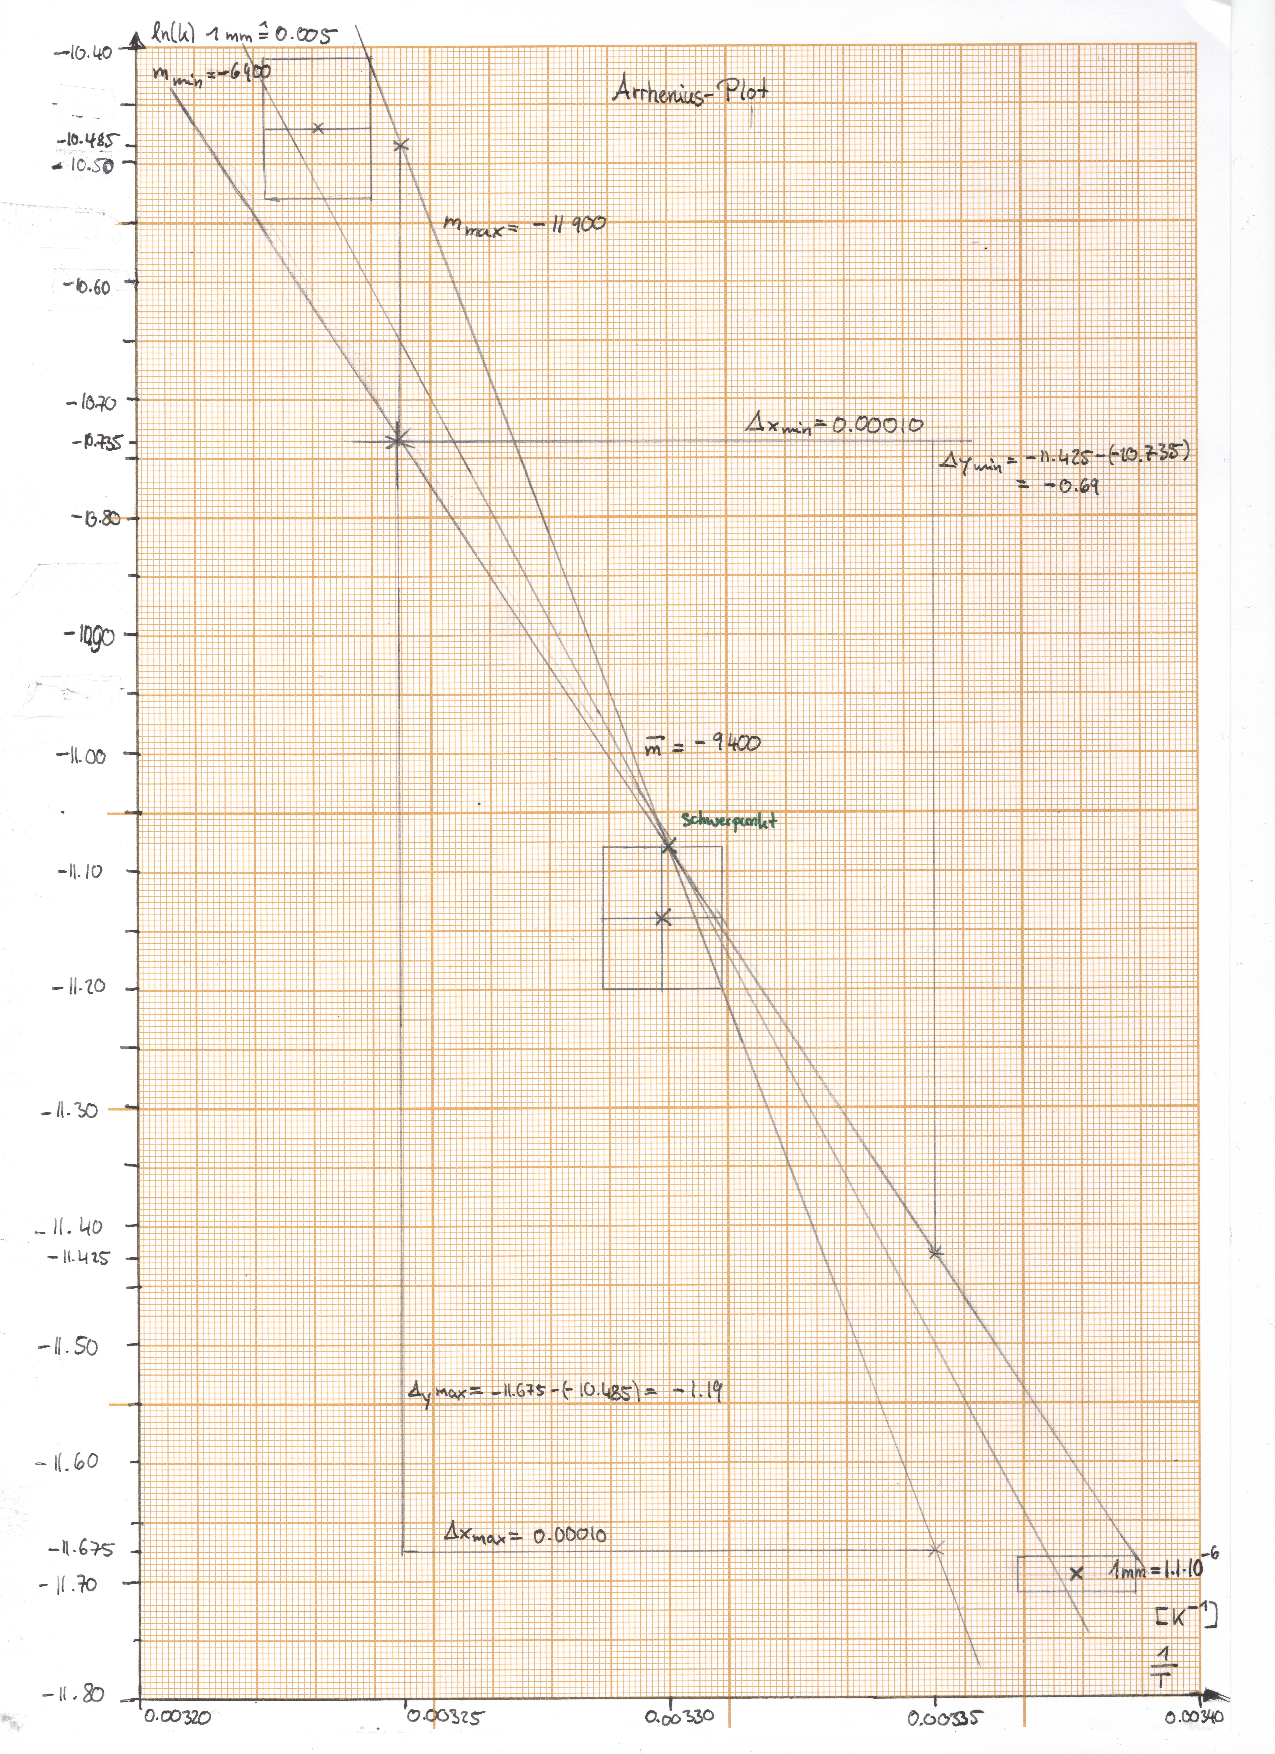
\includepdf{K3/Arrhenius.pdf}
